\documentclass[11pt]{article}
\usepackage[margin=1in]{geometry}
\usepackage[T1]{fontenc}
\usepackage[utf8]{inputenc}
\usepackage{lmodern}
\usepackage{microtype}
\usepackage[table]{xcolor}
\usepackage{amsmath,amssymb,amsfonts,mathtools,bm}
\IfFileExists{physics.sty}{%
  \usepackage{physics}%
}{%
  % Portable subset used by this project when the optional physics package
  % is not installed in the local TeX distribution.
  \NewDocumentCommand{\pdv}{o m m}{%
    \IfNoValueTF{##1}{\frac{\partial ##2}{\partial ##3}}%
    {\frac{\partial^{##1} ##2}{\partial ##3^{##1}}}%
  }
  \NewDocumentCommand{\dv}{o m m}{%
    \IfNoValueTF{##1}{\frac{\mathrm{d} ##2}{\mathrm{d} ##3}}%
    {\frac{\mathrm{d}^{##1} ##2}{\mathrm{d} ##3^{##1}}}%
  }
  \providecommand{\dd}{\mathop{}\!\mathrm{d}}
  \providecommand{\grad}{\nabla}
  \providecommand{\abs}[1]{\left\lvert ##1\right\rvert}
  \providecommand{\norm}[1]{\left\lVert ##1\right\rVert}
  \providecommand{\ket}[1]{\left\lvert ##1\right\rangle}
  \providecommand{\bra}[1]{\left\langle ##1\right\rvert}
}
\usepackage{booktabs,array,longtable,tabularx}
\usepackage{hyperref}
\usepackage{enumitem}
\usepackage{fancyhdr}
\usepackage{titlesec}
\usepackage{tcolorbox}
\usepackage{ragged2e}
\usepackage{setspace}
\IfFileExists{siunitx.sty}{%
  \usepackage{siunitx}%
}{%
  % Minimal text-safe fallback for the small number of \SI and \si calls in
  % this repository. Full siunitx formatting is used when available.
  \providecommand{\si}[1]{\ensuremath{\mathrm{##1}}}
  \providecommand{\SI}[2]{\ensuremath{##1\,\mathrm{##2}}}
}
\hypersetup{colorlinks=true, linkcolor=blue!50!black, urlcolor=blue!50!black, citecolor=blue!50!black}
\definecolor{TitleBlue}{HTML}{163A5F}
\definecolor{AccentTeal}{HTML}{2D6F73}
\definecolor{SoftBlue}{HTML}{EAF3F8}
\definecolor{SoftTeal}{HTML}{EDF8F6}
\definecolor{SoftGray}{HTML}{F5F7FA}
\definecolor{RuleGray}{HTML}{D7DEE8}
\pagestyle{fancy}
\fancyhf{}
\lhead{RadiationEffects\_proj2}
\rhead{Technical Notes}
\cfoot{\thepage}
\setlength{\headheight}{14pt}
\setlength{\parskip}{0.5em}
\setlength{\parindent}{0pt}
\onehalfspacing
\numberwithin{equation}{section}
\titleformat{\section}{\Large\bfseries\color{TitleBlue}}{\thesection}{0.6em}{}
\titleformat{\subsection}{\large\bfseries\color{AccentTeal}}{\thesubsection}{0.6em}{}
\titleformat{\subsubsection}{\normalsize\bfseries\color{TitleBlue}}{\thesubsubsection}{0.6em}{}
\newtcolorbox{overviewbox}{colback=SoftBlue,colframe=TitleBlue,boxrule=0.8pt,arc=2mm,left=3mm,right=3mm,top=2mm,bottom=2mm}
\newtcolorbox{physicsbox}{colback=SoftTeal,colframe=AccentTeal,boxrule=0.8pt,arc=2mm,left=3mm,right=3mm,top=2mm,bottom=2mm}
\newtcolorbox{notebox}{colback=SoftGray,colframe=AccentTeal,boxrule=0.6pt,arc=2mm,left=3mm,right=3mm,top=2mm,bottom=2mm}
\newcommand{\DocTitle}[3]{%
\begin{center}
{\LARGE \bfseries \color{TitleBlue} #1}\\[0.5em]
{\large \color{AccentTeal} #2}\\[0.8em]
{\normalsize #3}
\end{center}
\vspace{0.5em}}
\newenvironment{symtable}{\rowcolors{2}{SoftGray}{white}\begin{longtable}{>{\RaggedRight\arraybackslash}p{0.18\textwidth} >{\RaggedRight\arraybackslash}p{0.25\textwidth} >{\RaggedRight\arraybackslash}p{0.47\textwidth}}\toprule \textbf{Symbol / acronym} & \textbf{Name} & \textbf{Meaning in this document} \\ \midrule\endfirsthead\toprule \textbf{Symbol / acronym} & \textbf{Name} & \textbf{Meaning in this document} \\ \midrule\endhead}{\bottomrule\end{longtable}}


\newcommand{\ProjectTOC}{%
\vspace{0.6em}
{\hypersetup{linkcolor=TitleBlue,urlcolor=TitleBlue,citecolor=TitleBlue}\tableofcontents}
\vspace{1.0em}}

\newcommand{\SymbolsAcronymsSection}{%
\section*{Symbols and acronyms used in this document}%
\addcontentsline{toc}{section}{Symbols and acronyms used in this document}}

\newcommand{\rvec}{\bm{r}}
\newcommand{\qvec}{\bm{q}}
\newcommand{\nvec}{\bm{n}}
\newcommand{\xvec}{\bm{x}}
\newcommand{\kB}{k_{\mathrm{B}}}
\newcommand{\qp}{\mathrm{qp}}
\newcommand{\JJ}{\mathrm{JJ}}
\newcommand{\mfp}{\Lambda}
\allowdisplaybreaks

\usepackage{graphicx}
\usepackage{parskip}
\usepackage{tikz}
\usetikzlibrary{arrows.meta,positioning}
\newcolumntype{Y}{>{\RaggedRight\arraybackslash}X}
\definecolor{accent}{HTML}{163A5F}
\definecolor{accent2}{HTML}{EAF3F8}
\definecolor{accent3}{HTML}{F5F7FA}
\allowdisplaybreaks
\newtcolorbox{keybox}{colback=SoftBlue,colframe=TitleBlue,boxrule=0.8pt,arc=2mm,left=3mm,right=3mm,top=2mm,bottom=2mm}
\newtcolorbox{notebox}{colback=SoftGray,colframe=AccentTeal,boxrule=0.6pt,arc=2mm,left=3mm,right=3mm,top=2mm,bottom=2mm}
\rhead{Project Plan}

\begin{document}

\DocTitle{Project Plan}{Radiation-Induced Defect Evolution and Device Degradation in Silicon}{Single living roadmap for project architecture, workflow, file map, and module sequencing}

\begin{keybox}
\textbf{Purpose.} This document is the single living roadmap for \textbf{Radiation Effects Project 2}. The top-level \texttt{README.md}, \texttt{project\_plan.tex}, and \texttt{project\_plan.pdf} are the maintained architecture documents and should be updated whenever the project architecture changes.
\end{keybox}

\ProjectTOC

\begin{notebox}
\textbf{Current architecture revision.} Module 1 remains the Geant4 deposition module. Modules 2--6 are now 2D-first. Module 4 is split into \textbf{Module 4a} (continuum heat-equation thermal transport) and \textbf{Module 4b} (phonon-aware thermal transport). Module 7 remains the scaling and multiscale-prediction module.
\end{notebox}

\section{Project objective}
The project builds a physics-based framework for connecting a radiation event in silicon to the eventual degradation of device performance. The goal is not only to model where energy is deposited, but also to understand how that deposited energy creates defects, how those defects evolve with time and temperature, how they alter the internal electric fields and carrier transport, and ultimately how they change the behavior of the device.

The intended physics chain is:
\begin{enumerate}[leftmargin=1.6em]
    \item incident radiation deposits energy in silicon,
    \item deposited energy seeds point defects and effective defect populations,
    \item defects migrate, react, cluster, dissociate, and anneal,
    \item charged defects alter the internal electrostatic landscape,
    \item thermal evolution changes defect kinetics and transport coefficients,
    \item the changed field and trap population alter carrier transport,
    \item the coupled system produces measurable device degradation.
\end{enumerate}

\section{Module roadmap}
\begin{longtable}{p{0.08\linewidth} p{0.30\linewidth} p{0.52\linewidth}}
\toprule
\textbf{No.} & \textbf{Module} & \textbf{Purpose}\\
\midrule
1 & Geant4 radiation energy deposition in silicon & Compute where, when, and how much energy is deposited in silicon by the incident radiation field. Export a deposition map that seeds later damage or defect-generation models.\\
2 & Two-dimensional electrostatics with defect-dependent space charge & Solve the 2D electrostatic problem for a damaged silicon structure. Convert dopants and charged defects into electric potential, electric field, and depletion-structure changes.\\
3 & Two-dimensional defect evolution: diffusion, reaction, migration, and annealing & Evolve vacancies, interstitials, complexes, and effective defect species in 2D as functions of time and temperature.\\
4a & Two-dimensional continuum thermal transport & Solve the baseline temperature field with the continuum heat equation and use it to update diffusion coefficients, reaction rates, annealing rates, and other temperature-dependent physics.\\
4b & Two-dimensional phonon-aware thermal transport & Extend the thermal model beyond a plain bulk conductivity by incorporating phonon-mediated transport ideas, defect-dependent thermal transport, and reduced nonequilibrium or size-effect corrections when they materially affect the prediction.\\
5 & Two-dimensional drift-diffusion carrier transport with defect-assisted recombination & Predict how the damaged device transports electrons and holes under the altered field, temperature, and trap landscape.\\
6 & Coupled two-dimensional multiphysics degradation model & Couple Modules 2, 3, 4a/4b, and 5 into a self-consistent simulator for defect evolution, field evolution, thermal evolution, and carrier-transport degradation.\\
7 & Multiscale extrapolation and scalable prediction & Develop methods for making predictions on much larger spatial, temporal, or statistical scales than the direct high-fidelity simulation can afford. This module covers controlled approximations, quantified error bars, statistical upscaling, and hybrid multiresolution workflows.\\
\bottomrule
\end{longtable}

\section{Project narrative and module descriptions}
\textbf{Radiation-Induced Defect Evolution and Device Degradation in Silicon}

This project builds a physics-based framework for connecting a radiation event in silicon to the eventual degradation of device performance. The goal is not only to model where energy is deposited, but also to understand how that deposited energy creates defects, how those defects evolve with time and temperature, how they alter the internal electric fields and carrier transport, and ultimately how they change the behavior of the device. Each module isolates one layer of the physics, while the final module combines them into a self-consistent multiphysics model.

\textbf{Module 1. Geant4: Radiation Energy Deposition in Silicon}

This module provides the radiation input to the rest of the framework. Using Geant4, the simulation tracks incoming radiation and calculates where, when, and how much energy is deposited inside the silicon. The output of this step represents the initial physical insult to the material. In practice, this module gives the spatial and possibly temporal distribution of deposited energy that can later be translated into an initial defect-generation source term or damage map.

\textbf{Module 2. Electrostatics with Defect-Dependent Space Charge in a 2D Silicon Device Cross Section}

This module models how radiation-induced defects modify the electrostatic state of the device in two spatial dimensions. Defects can act as charged centers, traps, or ionized states that contribute to the net space-charge density. That altered space charge changes the electric potential and electric field inside the device. Physically, this matters because the internal field controls depletion behavior, carrier motion, and ultimately how the device responds under bias. This module therefore connects the evolving defect population to the device's internal field structure.

\textbf{Module 3. Two-Dimensional Diffusion-Reaction Solver for Defect Migration and Annealing}

This module describes the time evolution of radiation-induced defects after they are created. Defects are not static: they can diffuse, recombine, cluster, dissociate, or anneal depending on temperature and local conditions. A 2D diffusion-reaction model captures these mechanisms by evolving defect concentrations in space and time. This is one of the core physics modules of the project because it determines how initial damage develops into a changing defect landscape, rather than treating radiation damage as frozen in place.

\textbf{Module 4a. Two-Dimensional Continuum Thermal Transport}

This module adds temperature as an active physical driver using the continuum heat equation. Temperature influences defect mobility, reaction rates, and annealing kinetics, so the defect-evolution problem is inherently thermally sensitive. Module 4a calculates the baseline temperature field in the device, and that temperature field feeds into the defect-evolution equations. This branch is the production baseline because it is simpler, cheaper, and easier to validate.

\textbf{Module 4b. Two-Dimensional Phonon-Aware Thermal Transport}

This module is the richer thermal comparison branch. It retains the same project role as Module 4a but tries to represent heat transport in silicon more faithfully when phonon-mediated transport, defect scattering, size effects, or reduced nonequilibrium corrections matter. Module 4b exists so the project can test whether these additional thermal-transport effects change the quantities of interest enough to justify the extra complexity.

\textbf{Module 5. Two-Dimensional Drift-Diffusion Carrier Transport with Defect-Assisted Recombination}

This module translates material damage into electrical performance changes. Using 2D drift-diffusion transport equations, the model solves for electron and hole motion under the influence of the internal electric field and carrier concentration gradients. Radiation-induced defects enter through trap-assisted recombination, trapping, and lifetime degradation. In other words, this module shows how the evolving defect population, altered electrostatics, and temperature field affect measurable device behavior such as leakage current, charge collection, recombination losses, or degraded diode response.

\textbf{Module 6. Combined Multiphysics Model Using Modules 2, 3, 4a/4b, and 5}

This module integrates the previous physics pieces into a coupled framework. The defect population changes the space charge; the space charge changes the electric field; the electric field influences carrier transport; the temperature affects defect migration and annealing; and carrier behavior and local power dissipation can in turn interact with the thermal state. This module is where the project becomes a true device-degradation simulator rather than a collection of separate models. Its purpose is to produce a self-consistent prediction of how radiation exposure evolves into long-term electrical degradation.

\textbf{Module 7. Multiscale Extrapolation and Scalable Prediction}

This module addresses the fact that direct high-fidelity simulations may be too expensive for large devices, long times, broad parameter sweeps, or population-level reliability predictions. It covers controlled reduced-fidelity approximations, statistical upscaling, and hybrid multiresolution workflows. A central requirement is that any speedup or approximation be accompanied by a quantitative error metric relative to a higher-fidelity reference.

\section{Core architecture decision: 2D for Modules 2--6}
The original one-dimensional path was numerically attractive, but it suppresses several effects that become important once the damage pattern is spatially structured: lateral spreading of defect populations, lateral field bending, nonuniform temperature fields near localized energy deposition, and current crowding or carrier-flow rerouting. A 2D architecture is therefore the more faithful bridge between a realistic Geant4 source pattern and later electrostatic, thermal, and transport calculations.

This move to 2D does not mean every solver should start maximally complex. The first versions should still keep simple rectangular domains, structured grids, small defect networks, simple boundary conditions, and weak one-way coupling before self-consistent feedback.

\section{Run-order workflow for the project}
The run order below is the logical flow of a coupled study.

\begin{center}
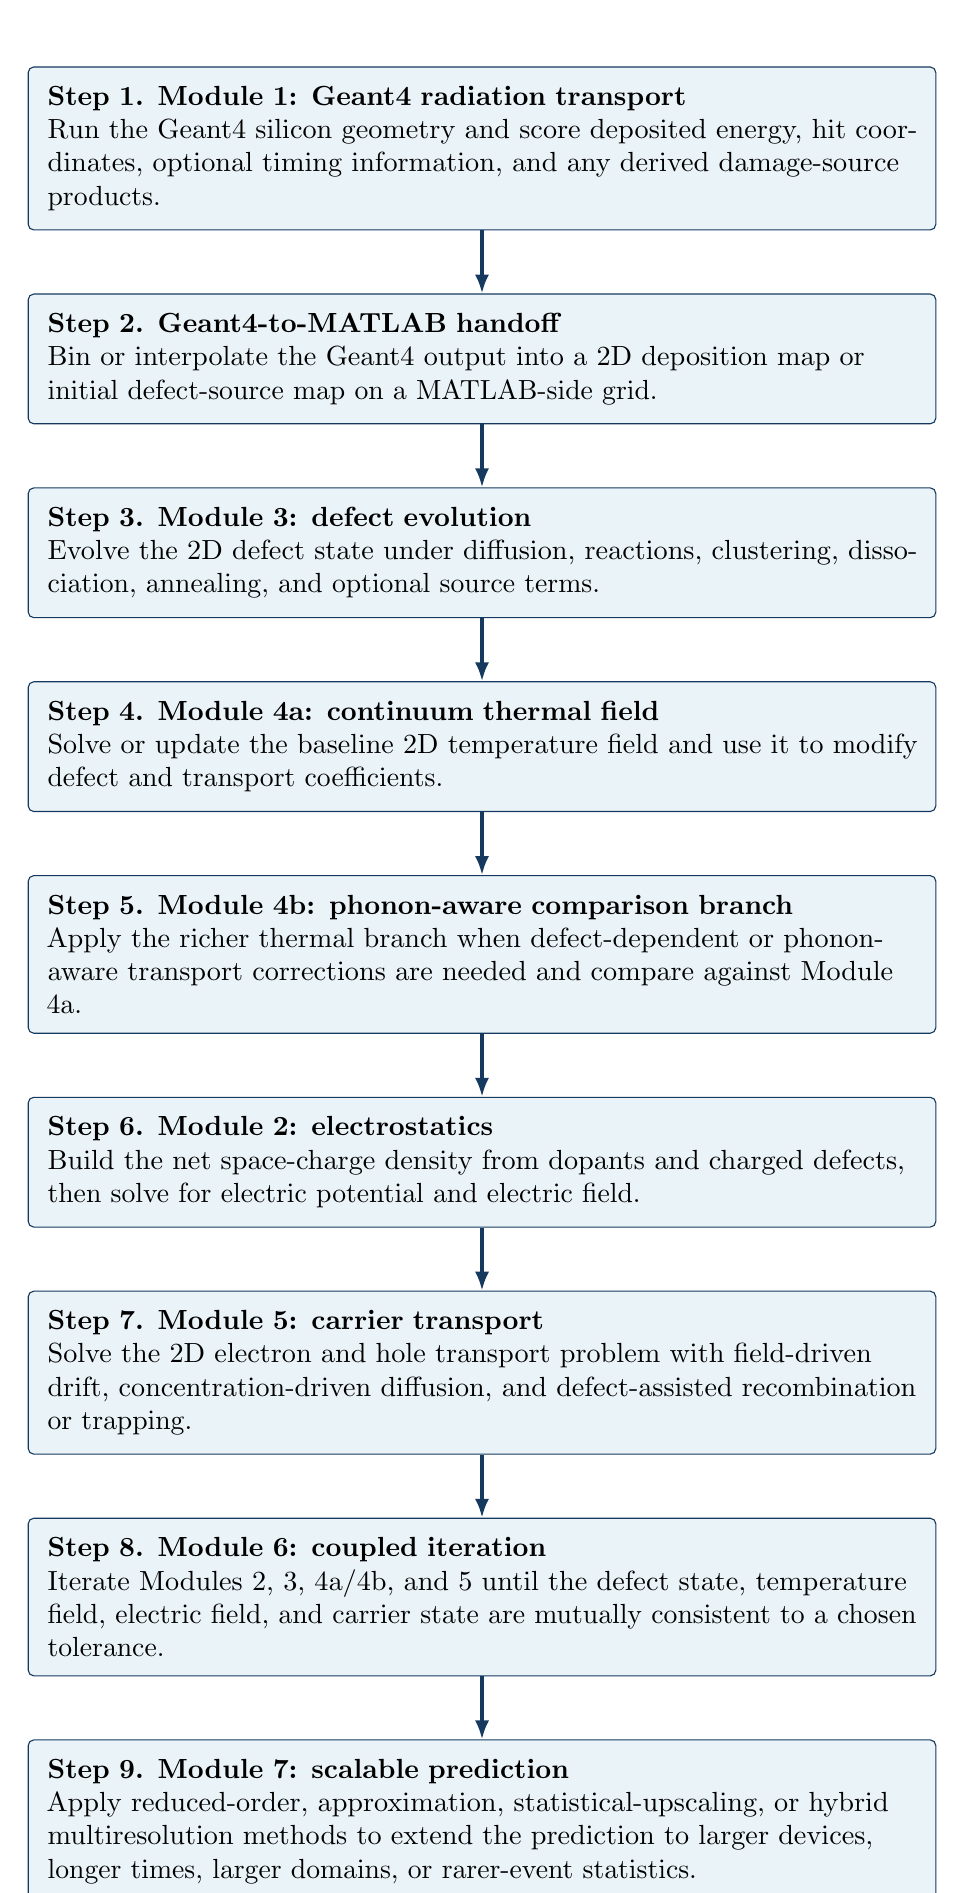
\begin{tikzpicture}[
node distance=8mm and 6mm,
box/.style={draw=accent, rounded corners=2pt, fill=accent2, minimum width=0.91\linewidth, text width=0.91\linewidth, align=left, inner sep=7pt},
arrow/.style={-{Latex[length=2.4mm]}, very thick, draw=accent}
]
\node[box] (m1) {\textbf{Step 1. Module 1: Geant4 radiation transport}\\Run the Geant4 silicon geometry and score deposited energy, hit coordinates, optional timing information, and any derived damage-source products.};
\node[box, below=of m1] (handoff) {\textbf{Step 2. Geant4-to-MATLAB handoff}\\Bin or interpolate the Geant4 output into a 2D deposition map or initial defect-source map on a MATLAB-side grid.};
\node[box, below=of handoff] (m3) {\textbf{Step 3. Module 3: defect evolution}\\Evolve the 2D defect state under diffusion, reactions, clustering, dissociation, annealing, and optional source terms.};
\node[box, below=of m3] (m4a) {\textbf{Step 4. Module 4a: continuum thermal field}\\Solve or update the baseline 2D temperature field and use it to modify defect and transport coefficients.};
\node[box, below=of m4a] (m4b) {\textbf{Step 5. Module 4b: phonon-aware comparison branch}\\Apply the richer thermal branch when defect-dependent or phonon-aware transport corrections are needed and compare against Module 4a.};
\node[box, below=of m4b] (m2) {\textbf{Step 6. Module 2: electrostatics}\\Build the net space-charge density from dopants and charged defects, then solve for electric potential and electric field.};
\node[box, below=of m2] (m5) {\textbf{Step 7. Module 5: carrier transport}\\Solve the 2D electron and hole transport problem with field-driven drift, concentration-driven diffusion, and defect-assisted recombination or trapping.};
\node[box, below=of m5] (m6) {\textbf{Step 8. Module 6: coupled iteration}\\Iterate Modules 2, 3, 4a/4b, and 5 until the defect state, temperature field, electric field, and carrier state are mutually consistent to a chosen tolerance.};
\node[box, below=of m6] (m7) {\textbf{Step 9. Module 7: scalable prediction}\\Apply reduced-order, approximation, statistical-upscaling, or hybrid multiresolution methods to extend the prediction to larger devices, longer times, larger domains, or rarer-event statistics.};
\draw[arrow] (m1) -- (handoff);
\draw[arrow] (handoff) -- (m3);
\draw[arrow] (m3) -- (m4a);
\draw[arrow] (m4a) -- (m4b);
\draw[arrow] (m4b) -- (m2);
\draw[arrow] (m2) -- (m5);
\draw[arrow] (m5) -- (m6);
\draw[arrow] (m6) -- (m7);
\end{tikzpicture}
\end{center}

\begin{notebox}
\textbf{Important distinction.} Module 4a is the baseline thermal branch and should be built first. Module 4b is a comparison branch rather than the first production dependency. In simplified studies, thermal information does not always have to be solved before electrostatics, but in the intended coupled workflow the temperature field should be available before the tightly coupled 2D solve because temperature changes diffusion, annealing, mobility, and recombination parameters.
\end{notebox}

\section{Recommended coding order}
\begin{enumerate}[leftmargin=1.6em]
    \item \textbf{Module 1:} Geant4 geometry, scoring, and export format.
    \item \textbf{Module 3:} 2D defect evolution on a structured grid.
    \item \textbf{Module 2:} 2D electrostatics with prescribed charged defects.
    \item \textbf{Module 4a:} 2D continuum thermal solver plus temperature-dependent coefficients.
    \item \textbf{Module 4b:} reduced phonon-aware thermal extension after the continuum baseline is working.
    \item \textbf{Module 5:} 2D drift-diffusion with prescribed electrostatic field, thermal field, and defect/trap fields.
    \item \textbf{Module 6:} weak coupling, then stronger feedback and iterative convergence.
    \item \textbf{Module 7:} scalable-prediction methods after at least one credible high-fidelity coupled workflow exists.
\end{enumerate}

\section{File-map overview}
\begin{longtable}{p{0.30\linewidth} p{0.60\linewidth}}
\toprule
\textbf{Path} & \textbf{Role}\\
\midrule
\path{README.md} & Public repository summary and high-level entry point.\\
\path{project_plan.tex/.pdf} & Single living roadmap document: project objective, module definitions, run order, file map, interfaces, and roadmap updates.\\
\path{docs/physics_notes/} & One large physics note per module, with derivations, symbol definitions, assumptions, and physical interpretation.\\
\path{docs/implementation_notes/} & Module-by-module implementation specifications, solver notes, and interface notes.\\
\path{geant4/} & Geant4-side setup, macros, and example outputs for Module 1.\\
\path{matlab/} & MATLAB drivers, source code, tests, outputs, and cross-module interfaces for Modules 2--7.\\
\bottomrule
\end{longtable}

\subsection{Current MATLAB map plus planned 2D emphasis}
\begin{longtable}{p{0.34\linewidth} p{0.57\linewidth}}
\toprule
\textbf{Path} & \textbf{Role in the updated 2D plan}\\
\midrule
\path{matlab/main_module2_electrostatics.m} & Top-level entry for the 2D electrostatic solve.\\
\path{matlab/main_module3_2d_defect_evolution.m} & Top-level entry for the 2D defect-evolution solve.\\
\path{matlab/main_module4a_2d_continuum_thermal.m} & Top-level entry for the Module 4a 2D continuum thermal solve.\\
\path{matlab/main_module4b_phonon_aware_thermal.m} & Planned top-level entry for the Module 4b phonon-aware thermal comparison branch.\\
\path{matlab/main_module5_drift_diffusion.m} & Top-level entry for the 2D carrier-transport solve.\\
\path{matlab/main_module6_multiphysics.m} & Top-level coupled driver that orchestrates Modules 2, 3, 4a/4b, and 5.\\
\path{matlab/src/grid/} & Shared 2D grid generation and spatial operators.\\
\path{matlab/src/module3_defects/} & Module 3 defect evolution operators and initialization helpers.\\
\path{matlab/src/module4a_thermal/} & Module 4a thermal operators, initialization helpers, and source-term assembly for the baseline continuum branch.\\
\path{matlab/src/electrostatics/} & Planned 2D Poisson operators, charge assembly, and field postprocessing.\\
\path{matlab/src/transport/} & Planned drift-diffusion operators, recombination models, mobility models, and current extraction.\\
\path{matlab/src/diagnostics/} & Shared diagnostics, error metrics, and summary writers.\\
\path{matlab/src/io/} & Shared I/O helpers and history save utilities.\\
\path{matlab/src/plot/} & Shared 2D visualization and history plotting utilities.\\
\path{matlab/tests/} & Verification problems and regression tests, including limiting-case checks.\\
\path{matlab/outputs/} & Saved run products, plots, summaries, and histories.\\
\bottomrule
\end{longtable}

\section{Thermal split rationale and comparison strategy}
\subsection{Module 4a: why it comes first}
Module 4a is the baseline production branch because it uses the continuum heat equation, is simpler to verify, and gives the temperature field required by later modules with minimal additional modeling assumptions.

\subsection{Module 4b: what it must add}
Module 4b exists to capture situations in which heat transport is changed materially by phonon-mediated effects, defect scattering, size effects, or reduced nonequilibrium corrections. Module 4b should not be added merely because it is more detailed. It should be added because it changes the quantities of interest enough to matter.

\subsection{Recommended comparison metrics for 4a versus 4b}
At minimum, compare:
\begin{itemize}[leftmargin=1.5em]
    \item peak temperature,
    \item spatial temperature gradients,
    \item time history of temperature at hot spots,
    \item defect-diffusion or annealing coefficient changes induced by temperature,
    \item downstream changes in defect histories or electrical degradation metrics,
    \item added computational cost.
\end{itemize}
A useful rule is that Module 4b should earn its place by changing one or more project-level quantities of interest enough to justify the extra complexity.

\section{Module interfaces in the new 2D plan}
\subsection{Module 1 to Module 3 handoff}
The first strong interface should now be a 2D deposition or defect-source map. A minimal handoff object should contain coordinate arrays, a deposited-energy density field, optional time-resolved source information, and metadata describing bin width, device geometry, radiation case, and units.

\subsection{Module 3 to Module 2 handoff}
After a defect-evolution run, MATLAB should save at minimum coordinate arrays, effective defect fields, charged-defect density fields, trap-density fields, and time-history diagnostics for provenance.

\subsection{Module 2 and Module 4a/4b to Module 5 handoff}
Carrier transport should read electric potential $\phi(x,y)$, electric-field components $E_x(x,y)$ and $E_y(x,y)$, temperature $T(x,y)$, and trap or recombination parameters derived from the defect state.

\section{Verification strategy under the 2D architecture}
Each module needs at least one low-complexity verification path.

\begin{longtable}{p{0.14\linewidth} p{0.77\linewidth}}
\toprule
\textbf{Module} & \textbf{Verification logic}\\
\midrule
1 & Compare deposition trends against known silicon behavior and verify that the exported 2D binning is internally consistent.\\
2 & Use manufactured or symmetric charge configurations whose 2D potential and field patterns are physically obvious; verify sign conventions and boundary-condition behavior.\\
3 & Check pure diffusion, pure annealing, and symmetry-preserving source cases in 2D. Total inventory should behave correctly under the chosen boundaries.\\
4a & Recover known 2D heat-conduction behavior on simple rectangular domains with simple source terms and boundary conditions.\\
4b & Demonstrate that the phonon-aware branch reduces to the Module 4a limit when phonon corrections are turned off, and quantify when defect-dependent transport changes the result.\\
5 & Verify defect-free transport first, then turn on simple trap-assisted recombination. Check that zero-field or symmetric cases behave sensibly.\\
6 & Confirm that decoupled or weakly coupled limits reduce to standalone solutions. Track iterative residuals and relaxation behavior.\\
7 & Every scalable-prediction method must be benchmarked against a higher-fidelity reference. The benchmark should report both speedup and error metrics.\\
\bottomrule
\end{longtable}

\section{Module 7: multiscale extrapolation and scalable prediction}
A stronger title than ``scaling up methods of the simulation'' is \textbf{Multiscale Extrapolation and Scalable Prediction}. This module has three important branches:
\begin{enumerate}[leftmargin=1.6em]
    \item \textbf{Controlled reduced-fidelity approximation:} coarser meshes, simplified defect networks, operator splitting, or reduced-order models. These must be judged by both speedup and error relative to a higher-fidelity reference.
    \item \textbf{Statistical approximation and upscaling:} using smaller simulated tiles, event statistics, or surrogate source distributions to infer larger-scale behavior.
    \item \textbf{Hybrid multiresolution coupling:} high fidelity only in physically critical regions, with coarser or cheaper models elsewhere.
\end{enumerate}
A useful project-level trade plot is approximation error versus speedup rather than speed alone.

\section{When this project-plan document should be updated}
This document should be revised whenever a module definition changes, the dimensionality assumption changes, a new top-level file or folder becomes part of the standard workflow, an inter-module file format changes, the run order changes, a major verification strategy changes, or Module 7 gains a concrete benchmark or scaling method.

\section{Near-term next steps after this revision}
\begin{enumerate}[leftmargin=1.6em]
    \item Keep the top-level \texttt{README.md}, \texttt{project\_plan.tex}, and \texttt{project\_plan.pdf} synchronized whenever the project architecture changes.
    \item Verify the first 2D Module 3 code path on the user's MATLAB environment.
    \item Implement and verify the first Module 4a continuum thermal baseline in MATLAB.
    \item Define the first reduced phonon-aware closure path for Module 4b and the metrics it must change enough to justify the extra complexity.
    \item Update the Module 2, 4a/4b, and 5 implementation notes so their first solver architecture is 2D rather than 1D.
    \item Decide the first benchmark quantity of interest for Module 7 so that future approximations can be measured against something physically meaningful.
\end{enumerate}

\end{document}
